\documentclass[runningheads]{llncs}
%
\usepackage[T1]{fontenc}
\usepackage{lmodern}
\usepackage{graphicx}
\usepackage{paralist}
\usepackage{csquotes}
\usepackage{xspace}
\usepackage{tikz}
\usepackage{pgfplots}
\usepackage{tabularx}
\usepackage{ragged2e}
\usepackage{adjustbox}
\usepackage{microtype}
\usepackage{booktabs}
\usetikzlibrary{shapes,arrows,positioning,fit,backgrounds}
\pgfplotsset{compat=1.16}

\begin{document}
%
\title{Operationalizing Human-AI Collaboration for High-Volume Project Risk Management}
%
\titlerunning{Operationalizing Human-AI Collaboration for Project Risk Management}
%
\author{Marc Bara\inst{1,2}\orcidID{0009-0005-1480-5760}}
\authorrunning{Bara M.}
\institute{ICSO Analytics, Barcelona, Spain \and
ESADE Business School, Barcelona, Spain\\
\email{marcoantonio.bara@esade.edu}}
%
\maketitle
%

\begin{abstract}
Artificial intelligence tools can now generate hundreds of potential risk scenarios per project, creating an ``intelligence paradox'' where AI's analytical power overwhelms rather than assists project managers. In previous work~\cite{bara2025catania}, we identified four human-AI collaboration patterns from cybersecurity, security screening, financial systems, and robotics that address high-volume risk management, and proposed a theoretical transfer framework to project management. However, that framework remained at the conceptual level, leaving a critical gap between theory and implementation. This paper operationalizes the framework into SHARP (Semantic Human-AI Risk Prioritization), defining: (a) a semantic triage system where AI classifies risks through contextual understanding rather than traditional probability-impact matrices, (b) a three-tier collaboration model (MONITOR/FLAG/ESCALATE) with clearly delineated AI and human responsibilities, and (c) a four-layer safety architecture ensuring the system fails safely when---not if---classification errors occur. We present a simulation-based validation using a synthetic project with planted ground-truth risks, processed through an LLM-based orchestration pipeline. The system is designed so that the project manager defines semantic classification rules while AI executes them at volume---preserving human judgment where it matters while delegating volume processing to AI.

\keywords{project risk management \and human-AI collaboration \and decision support systems \and semantic risk triage \and LLM orchestration \and safe failure \and human-AI teaming}
\end{abstract}

\section{Introduction}

Project risk management faces a paradox. As AI tools become capable of analyzing project plans, communications, and historical data to identify potential risks, they can generate hundreds of risk scenarios for a single project---far exceeding any project manager's capacity to evaluate manually. We term this the \emph{intelligence paradox}: AI's analytical power, naively applied, creates more information overload than it solves~\cite{bara2025catania}. This challenge sits at the core of human-AI collaboration for real-world decision-making: how to leverage AI's processing capacity without sacrificing the contextual judgment that makes risk management effective.

This is not a hypothetical concern. Our prior systematic review~\cite{bara2025catania} examined 344 papers across two search streams: 296 on AI-related project management challenges and 48 on human-AI collaboration frameworks in adjacent high-volume domains. Of the 296 PM-focused papers, 17 already document information overload challenges~\cite{annexure2024,km2024,aidecision2025,responsibleai2024}, yet none propose systematic solutions adapted from domains that have already solved analogous problems.

This paper builds on two complementary prior lines of work. \cite{bara2025catania} (the ``Catania'' framework) identified four human-AI collaboration patterns from cybersecurity, security screening, financial systems, and robotics, mapped them to PM challenges through a transfer matrix, articulated three adaptation principles (context preservation, threshold calibration, integration requirements), and proposed a three-tier threshold system (MONITOR/FLAG/ESCALATE)---but at the conceptual level, leaving the operational design unspecified. In parallel, \cite{bara2025augmenting} demonstrated that an LLM-based pipeline can detect semantic deficiencies in risk register entries and reformulate them at scale, but applied a single uniform treatment to every risk: it had no triage, no tier-based delegation, no clustering, no longitudinal reclassification, and no safety architecture against misclassification.

SHARP (Semantic Human-AI Risk Prioritization) operationalizes Catania's framework while extending the LLM pipeline of~\cite{bara2025augmenting} into a triage-aware system. Our contributions are threefold. First, we define a \textbf{semantic triage system} where risk classification is based on contextual understanding rather than numerical probability-impact scoring. Second, we specify the \textbf{precise responsibilities} of AI and human at each tier, including how the project manager configures the system through semantic rules and how the AI executes those rules at volume. Third, we develop a \textbf{four-layer safety architecture} that ensures the system fails safely when classification errors occur. We also present a simulation-based validation study with planted ground-truth criticals.

\section{Background: From Cross-Domain Patterns to SHARP}

Our previous systematic review~\cite{bara2025catania} established that successful human-AI collaboration in high-volume risk contexts follows distinct patterns. Four were identified and mapped to project management challenges through a transfer matrix (Table~\ref{tab:patterns}).

\begin{table}[htbp]
\caption{Collaboration patterns identified in~\cite{bara2025catania} and their PM adaptation}
\label{tab:patterns}
\begin{tabularx}{\textwidth}{|p{2.2cm}|p{2.2cm}|>{\raggedright\arraybackslash}X|>{\raggedright\arraybackslash}X|}
\hline
\textbf{Pattern} & \textbf{Source Domain} & \textbf{Core Logic} & \textbf{PM Adaptation} \\
\hline
Alert Prioritization~\cite{alertpriority2024} & Cybersecurity & AI clusters thousands of alerts to surface attack patterns & AI identifies risk clusters and dangerous combinations \\
\hline
Dual-Strategy Triage~\cite{humanloop2025} & Security Screening & Clear/flag/escalate classification of items & AI auto-clears low risks, escalates those needing human judgment \\
\hline
Weak-Signal Detection~\cite{weaksignal2022} & Financial Systems & Monitor data streams for early warning signs & AI scans project communications for emerging risk indicators \\
\hline
Multi-Unit Coordination~\cite{robotmission2024} & Robotics & Aggregate status data across units, suggest reallocation & AI consolidates cross-team risks, identifies conflicts \\
\hline
\end{tabularx}
\end{table}

The framework also proposed three adaptation principles: \emph{context preservation} (project risks are context-dependent, unlike universal cybersecurity threats), \emph{threshold calibration} (PM decisions often involve irreversible commitments, requiring conservative thresholds), and \emph{integration requirements} (the fragmented PM toolset landscape). A three-tier system was proposed: AI-managed monitoring for low-severity risks, AI-flagged human review for moderate risks, and direct human intervention for high-severity risks. This paper operationalizes that system into SHARP.

\section{Operationalizing SHARP}

The operationalization of SHARP addresses three questions left open by the theoretical framework: how classification decisions are made, what each actor does at each tier, and how the system adapts as the project evolves.

\subsection{Semantic Rules: The Human Configures, the AI Executes}

A fundamental design decision distinguishes this approach from traditional risk matrices~\cite{acebes2024}: classification is based on \textbf{semantic rules defined by the project manager}, not on numerical probability-impact scores.

At project initiation, the PM configures the system with rules expressed in natural language:
\begin{itemize}
    \item ``Anything affecting the critical path within 4 weeks $\to$ minimum FLAG''
    \item ``More than one risk linked to the same supplier $\to$ FLAG''
    \item ``Any risk affecting client relationship $\to$ ESCALATE''
    \item ``If the AI has low confidence in its assessment $\to$ FLAG, never MONITOR''
    \item ``During weeks 8--12 (critical phase) $\to$ lower all thresholds''
\end{itemize}

These rules encode the PM's contextual knowledge---their understanding of stakeholders, organizational dynamics, and strategic priorities. The AI cannot generate these rules; this is the irreplaceable human contribution. However, once defined, a large language model (LLM) can interpret and apply them at scale across hundreds of risks simultaneously.

This design directly implements the \emph{context preservation} principle from~\cite{bara2025catania}: the human retains strategic judgment by designing the policy; the AI handles volume execution.

\subsection{AI Semantic Reading}

For each risk, the AI performs a contextual semantic analysis rather than computing a numerical score. The LLM evaluates: (1)~the risk's semantic meaning and affected project components, (2)~connections with other risks that could create amplification, (3)~critical path proximity and timing margins, (4)~reversibility of impact if the risk materializes, (5)~corroborating signals in project communications, and (6)~the AI's own confidence in its assessment---where low confidence is itself a reason to escalate.

This semantic reading, combined with the PM's rules, determines tier classification. The distinction from traditional approaches is significant: a probability-impact matrix treats risks as independent data points with numerical coordinates, while semantic reading treats each risk as a contextualized narrative within the broader project story.

\textbf{Confidence is self-reported in the structured output.} The Analyst's prompt constrains the response to a JSON schema in which every classification carries a \texttt{confidence} field on $[0,1]$ alongside its tier and justification. The model is instructed to interpret this field as its self-assessed confidence in the tier choice given the semantic content and the PM rules, and the system prompt explicitly states that ``if AI confidence is low (below a documented threshold), classify FLAG, never MONITOR.'' This makes low confidence a first-class architectural trigger rather than a post-hoc inspection: the safety rule operates inside the classification call. We chose self-reported confidence over alternatives such as log-probability calibration or a secondary verifier because it composes cleanly with structured output, it is interpretable in the same prose vocabulary the PM uses to write rules, and the empirical results (Section~\ref{sec:results}) show the expected ordering---ESCALATE confidence highest, FLAG lowest, MONITOR intermediate---which supports its diagnostic value.

\subsection{Three-Tier Collaboration Model}

\textbf{Tier~1---MONITOR (AI decides, PM defines rules).} When the semantic reading indicates low impact, no critical path connection, no match with PM escalation rules, high reversibility, and high AI confidence, the system automatically assigns ``accept and monitor.'' This is the only tier where the AI makes the response decision autonomously. Crucially, the AI continuously re-evaluates these risks with every new project event, reclassifying upward if context changes. Expected volume: approximately 65--70\%. The rationale mirrors cybersecurity operations, where analysts configure rules for auto-closure of low-priority alerts rather than reviewing each one individually~\cite{alertpriority2024}.

\textbf{Tier~2---FLAG (AI proposes, PM decides).} Triggered by moderate impact, high uncertainty, a match with PM escalation rules, low AI confidence, or cluster membership. The AI proposes a concrete response with semantic justification---e.g., ``mitigate by renegotiating the timeline with Supplier~X, because this risk amplifies Risk~\#47 and both converge in Week~12.'' The PM reviews, applies contextual knowledge (political relationships, contractual constraints, sponsor tolerance), and accepts, modifies, or rejects. Expected volume: approximately 20--25\%.

\textbf{Tier~3---ESCALATE (AI informs, PM acts with team).} Reserved for high impact on project objectives, low reversibility, systemic threats from multiple connected risks, or PM direct escalation rules (client relationship, safety, compliance). The AI prepares a complete dossier but does \emph{not} decide the response. The PM works on these with their team, stakeholders, and sponsors. Expected volume: approximately 5--10\%.

Table~\ref{tab:tiers} summarizes the collaboration model.

\begin{table}[htbp]
\caption{Three-tier collaboration model: AI and human responsibilities}
\label{tab:tiers}
\begin{tabularx}{\textwidth}{|p{1.8cm}|p{1.2cm}|>{\raggedright\arraybackslash}X|>{\raggedright\arraybackslash}X|>{\raggedright\arraybackslash}X|}
\hline
\textbf{Tier} & \textbf{Volume} & \textbf{AI Responsibility} & \textbf{PM Responsibility} & \textbf{Risk Response} \\
\hline
MONITOR & 65--70\% & Apply PM rules, classify, monitor, reclassify if context changes & None (unless promoted) & AI decides: accept + monitor \\
\hline
FLAG & 20--25\% & Propose response with semantic justification & Review, add context, decide & PM decides \\
\hline
ESCALATE & 5--10\% & Prepare complete dossier & Act with team, stakeholders & PM designs with team \\
\hline
\end{tabularx}
\end{table}

\subsection{Dynamic Reclassification}

Risks are not static. Every new project event triggers a reclassification cycle across the entire register. A MONITOR risk may be promoted to FLAG when clustering detects a new connection with another risk, or when a communication signal confirms a concern. A FLAG risk may be promoted to ESCALATE when multiple related risks converge. Conversely, an ESCALATE risk may be demoted to FLAG after the PM's response reduces the threat, and a FLAG risk may return to MONITOR if the underlying condition is resolved.

Additionally, the PM's phase-based rules activate dynamically. When the project enters a pre-defined critical phase, thresholds drop globally: risks that were classified as MONITOR may be automatically promoted to FLAG. This is not the AI deciding to become more cautious---it is the PM's pre-configured policy activating on schedule.

\textbf{Computational scope of a reclassification cycle.} For each project event, the orchestrator does not blindly re-evaluate every risk in the register. It computes an \emph{affected set} by intersecting the event with structural filters: risks sharing the same supplier, team, or critical-path segment as the event; existing FLAG/ESCALATE risks whose clusters could grow; and a rolling window of recent MONITOR risks that may have crossed a threshold. Only risks in the affected set are re-sent to the Analyst, batched to respect context-window limits. This bounds per-event cost from \(O(N)\) to roughly \(O(k)\) where \(k\) is the size of the affected set, typically a small fraction of the register in large projects. A full periodic re-evaluation can still be scheduled (e.g., weekly) as a safety net, but is not the per-event path. The minimal pipeline reported in Section~\ref{sec:results} exercises only the initial static classification; per-event filtered reclassification is left to follow-on work.

\section{Simulation-Based Validation Design}

To test whether SHARP produces a manageable, high-quality risk picture from an AI-generated risk explosion, we conduct a simulation study using a synthetic project with controlled ground truth.

\subsection{Synthetic Project with Planted Ground Truth}

We construct a synthetic project with multiple teams, vendors, and critical path dependencies. The project includes a complete plan (scope, schedule, WBS, organizational structure, budget, and an initial 20--30 risk register) and a timeline of 15--20 simulated events representing triggers that in production would arrive continuously---e.g., a supplier confirming a 5-day delay in Week~3, a technician emailing ``not sure we'll make the integration deadline'' in Week~4, a client-driven scope change in Week~6, and the project entering its critical path phase in Week~13.

Within the scenario, we plant ground-truth ``mines'': approximately 20--30 critical risks, 3--4 dangerous combinations invisible as individual risks but lethal together, 5--6 weak signals buried in simulated communications, and 2--3 interface gaps no single team owns. These constitute the ground truth against which SHARP is evaluated. The framework never has access to this ground truth; it must discover these risks through its own analysis.

\subsection{System Architecture}

The system consists of five components (Fig.~\ref{fig:architecture}): (1)~a \textbf{SQLite database} as single source of truth for all risks, classifications, justifications, and reclassification history; (2)~an \textbf{LLM Generator} that receives project inputs and produces risks in deliberately unfiltered batches---targeting approximately 500 from initial plan analysis alone; (3)~an \textbf{LLM Analyst} that applies the triage framework in batches of 30--50 risks (respecting context window constraints), performs clustering on FLAG/ESCALATE risks, scans communications for weak signals, and reclassifies existing MONITOR risks; (4)~a \textbf{Python orchestrator} managing the pipeline sequence; and (5)~a \textbf{Streamlit dashboard} for visualization.

\begin{figure}[htbp]
\centering
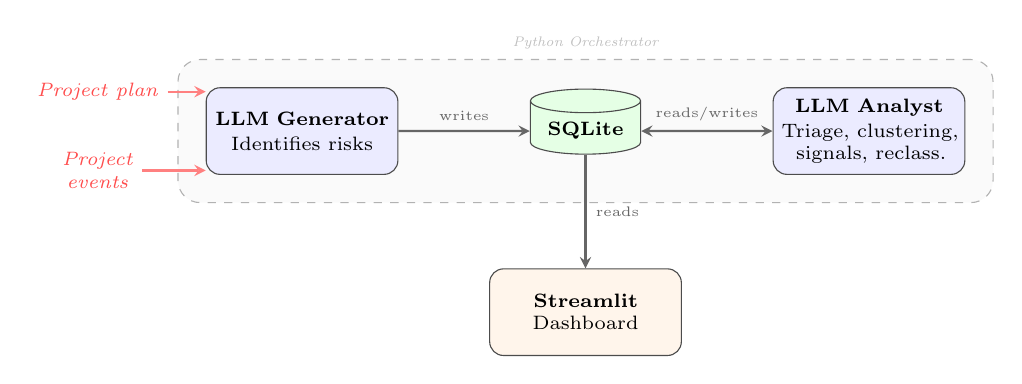
\begin{tikzpicture}[
    comp/.style={rectangle, rounded corners=5pt, draw=black!70, fill=blue!8, 
                 text width=2.2cm, minimum height=1.1cm, align=center, font=\scriptsize},
    db/.style={cylinder, draw=black!70, fill=green!10, minimum width=1.4cm, 
               minimum height=0.8cm, align=center, font=\scriptsize, shape border rotate=90, aspect=0.25},
    ui/.style={rectangle, rounded corners=5pt, draw=black!70, fill=orange!8, 
               text width=2.2cm, minimum height=1.1cm, align=center, font=\scriptsize},
    arrow/.style={->, >=stealth, thick, black!60},
    input/.style={font=\scriptsize\itshape, text=red!70, align=center}
]
    % Three main components in a row
    \node[comp] (gen) at (0, 0) {\textbf{LLM Generator}\\[1pt]Identifies risks};
    \node[db] (db) at (3.6, 0) {\textbf{SQLite}};
    \node[comp] (ana) at (7.2, 0) {\textbf{LLM Analyst}\\[1pt]Triage, clustering,\\signals, reclass.};

    % Orchestrator dashed box behind the three (on background layer)
    \begin{pgfonlayer}{background}
    \node[rectangle, rounded corners=8pt, draw=black!30, dashed, fill=gray!4,
          fit=(gen)(db)(ana), inner sep=10pt] (orch) {};
    \end{pgfonlayer}
    \node[font=\tiny\itshape, text=gray!50, anchor=south] at (orch.north) {Python Orchestrator};

    % Inputs above-left
    \node[input] (plan) at (-2.6, 0.5) {Project plan};
    \node[input] (events) at (-2.6, -0.5) {Project\\events};

    % Dashboard below-center
    \node[ui] (dash) at (3.6, -2.3) {\textbf{Streamlit}\\Dashboard};

    % Input arrows
    \draw[arrow, red!50] (plan.east) -- (gen.west |- plan.east);
    \draw[arrow, red!50] (events.east) -- (gen.west |- events.east);
    
    % Pipeline flow
    \draw[arrow] (gen.east) -- node[font=\tiny, above] {writes} (db.west);
    \draw[arrow, <->] (db.east) -- node[font=\tiny, above] {reads/writes} (ana.west);
    
    % DB to dashboard
    \draw[arrow] (db.south) -- node[font=\tiny, right] {reads} (dash.north);

\end{tikzpicture}
\caption{System architecture. The LLM Generator identifies risks from the project plan and subsequent events; the LLM Analyst reads risks from SQLite, applies triage, clustering, and signal scanning, and writes classifications back. A Python orchestrator (dashed) coordinates the pipeline. The dashboard reads from SQLite for visualization.}
\label{fig:architecture}
\end{figure}

For each simulated event, the orchestrator executes: (i)~feed the event to the Generator for new risks, (ii)~triage new risks, (iii)~reclassify existing MONITOR risks against new context, (iv)~cluster all FLAG/ESCALATE risks, (v)~scan communications for weak signals, and (vi)~update the database.

\textbf{Reproducibility.} The LLM pipeline inherits its plumbing from~\cite{bara2025augmenting}: the seven-field risk schema (Risk ID, Type, Root Cause, Incident, Impact, Response Strategy, Response Action), batch processing, and structured-output handling. SHARP extends this base in four ways: (a) replacing the single-task quality-enhancement prompt with a triage system prompt encoding the PM's semantic rules and tier definitions, (b) constraining the output via JSON-schema structured outputs to return \texttt{tier}, \texttt{confidence}, and \texttt{justification} per risk, (c) substituting SQLite for the CSV round-trip to support longitudinal analysis, and (d) adding ground-truth labels for evaluation. The Analyst runs on Claude Sonnet~4.6 with adaptive thinking disabled, effort set to \texttt{low}, and prompt caching enabled on the system block---the system prompt is identical across batches, so batches~2--N read from cache. The classification batch size is 20. The full system prompt, dataset, SQLite schema, and metrics code accompany the camera-ready version.

\textbf{Database schema.} The SQLite store uses three tables. The \texttt{risks} table holds one row per risk with the seven semantic fields (type, root cause, incident, impact, response strategy, response action, plus an optional \texttt{ground\_truth\_tier} used only for evaluation). The \texttt{classifications} table is append-only: each tier assignment generates a new row keyed by \texttt{risk\_id} with \texttt{tier}, \texttt{confidence}, \texttt{justification}, model identifier, timestamp, and optional \texttt{triggering\_event\_id}. This append-only design preserves the full reclassification history of each risk, enabling the longitudinal analysis required to study tier drift over the project lifecycle. The \texttt{events} table records project events that trigger reclassification cycles, with a foreign-key relationship into \texttt{classifications}.

\subsection{Evaluation Metrics}

The controlled ground truth enables precise measurement: \emph{critical risk retention rate} (planted critical risks correctly classified as FLAG/ESCALATE), \emph{volume reduction} (percentage classified as MONITOR), \emph{cluster detection accuracy} (identification of planted dangerous combinations), \emph{initial false negative rate} (critical risks wrongly sent to MONITOR on first pass), \emph{recovery rate} (false negatives correctly reclassified after subsequent events), and \emph{time to recovery} (events required for self-correction).

\subsection{Results}
\label{sec:results}

We report initial results from a minimal end-to-end execution of the pipeline: a single static classification pass over a synthetic project of 80 risks with planted ground truth (12 ESCALATE, 18 FLAG, 50 MONITOR). The full multi-event simulation with dynamic reclassification, clustering, and weak-signal scanning is deferred to follow-on work and the camera-ready extension; the static pass already exercises the core triage mechanism and the four-layer safety architecture.

\textbf{Headline metrics.} The system achieved a \textbf{critical retention rate of 100\%} (12/12 planted ESCALATE risks placed in FLAG or ESCALATE) and an \textbf{initial false-negative rate of 0\%}---no critical risk was silently routed to MONITOR. The \textbf{volume reduction to MONITOR was 66.2\%} (53/80 risks), within the 65--70\% range anticipated by the framework. Per-tier exact-match recall was MONITOR 50/50 = 100\%, FLAG 11/18 = 61.1\%, ESCALATE 12/12 = 100\%; overall exact-match accuracy was 73/80 = 91.2\%. Table~\ref{tab:confusion} reports the full confusion matrix.

\begin{table}[htbp]
\caption{Confusion matrix on the static classification pass (rows = planted ground truth, columns = AI classification)}
\label{tab:confusion}
\centering
\begin{tabular}{|l|r|r|r|}
\hline
\textbf{GT \textbackslash{} AI} & \textbf{MONITOR} & \textbf{FLAG} & \textbf{ESCALATE} \\
\hline
MONITOR  & 50 & 0  & 0  \\
\hline
FLAG     & 3  & 11 & 4  \\
\hline
ESCALATE & 0  & 0  & 12 \\
\hline
\end{tabular}
\end{table}

\textbf{Evidence of conservative bias (Layer~1).} Every classification error on the FLAG row went \emph{upward} (4 to ESCALATE) or to MONITOR for low-impact reversible items (3); no error crossed the boundary that the safety architecture is designed to prevent (a critical risk leaking into MONITOR). The 4 FLAG-to-ESCALATE over-escalations all involved triggers the PM rules explicitly flag for escalation: a production-incident-likely configuration drift, an SLA breach on enterprise contracts, vendor concentration across multiple risks, and a single point of failure in on-call coverage. These are defensible escalations rather than spurious noise, and they are consistent with the system being asymmetrically tuned to favor false positives over false negatives (Layer~1 of the safety architecture, Section~\ref{sec:discussion}).

\textbf{Confidence as a diagnostic signal.} Mean AI-reported confidence ordered as expected by design: ESCALATE 0.95, MONITOR 0.79, FLAG 0.75. The FLAG tier carrying the lowest confidence confirms that the model expresses genuine uncertainty in the ambiguous middle band, and supports the use of low confidence as a first-class trigger for human review (Layer~1, Section~\ref{sec:discussion}).

\textbf{Cost and baseline.} The full 80-risk classification ran in four batches of 20 against Claude Sonnet~4.6 with prompt caching on the system block; total cost was approximately US\$0.07 (batches 2--4 read the system prompt from cache at ${\sim}10\%$ of base input price). For comparison, the LLM-only baseline from~\cite{bara2025augmenting}---which uses the same model family on the same risk schema but without the triage architecture---returns a single undifferentiated list with no tier signal, no confidence calibration, and no safety-driven prioritization, leaving the PM with the same 80-risk review load that motivated this work. SHARP reduces that load to the 27 risks (FLAG + ESCALATE) the PM actively needs to attend to, while guaranteeing that the 12 planted criticals are inside that 27.

\section{Discussion: Reliability and Safe Failure}
\label{sec:discussion}

The question ``LLMs are unreliable---how can you trust risk classification to one?'' requires direct engagement. Our answer is not that the system is infallible, but that it is designed to \textbf{fail safely}, and that its failure mode is superior to current practice.

\textbf{The only dangerous error} is classifying a critical risk as MONITOR---because then no human examines it. Other errors are tolerable: a trivial risk classified as FLAG wastes minutes of PM time; a moderate risk classified as ESCALATE receives excess attention. The safety architecture specifically targets the dangerous error through four layers.

\textbf{Layer~1: Conservative bias.} The LLM Analyst is configured to classify upward when uncertain. Low confidence mandates FLAG, never MONITOR. This produces more false positives but fewer false negatives---the same asymmetry used in medical screening. \textbf{Layer~2: Continuous reclassification.} A wrongly classified MONITOR risk is re-evaluated with every project event; if genuinely critical, subsequent signals will promote it. \textbf{Layer~3: PM override rules.} For non-negotiable domains (safety, compliance, client relations), the PM blocks MONITOR classification entirely---the human sets the floor. \textbf{Layer~4: Transparency.} Every classification includes its justification; the PM can query and manually promote any MONITOR risk. The dashboard operationalizes this without overwhelming the PM by inverting the default visibility: the FLAG and ESCALATE queues are shown expanded with full justifications and confidence scores, while the MONITOR queue is collapsed to a count with on-demand drill-down. A PM who wants to audit MONITOR decisions can filter by confidence (showing low-confidence MONITOR risks first, where review is most warranted), by escalation-rule keyword, or by free-text search over the justifications. Manual override is a single click that creates a new row in the append-only \texttt{classifications} table, preserving the audit trail. The design principle is that transparency must be \emph{available} rather than \emph{forced}: the PM sees what needs attention by default, and can excavate the rest only when a specific question arises.

\textbf{Limitations.} Synthetic project data cannot fully capture organizational complexity---political dynamics, informal channels, and tool fragmentation in real environments. LLM outputs exhibit inherent variability; we mitigate this with several controls but it is not eliminated. Specifically, the Analyst runs with adaptive thinking disabled and effort set to low (the prompt is the primary lever, not the reasoning depth), the system prompt is version-controlled and the version hash is stored alongside each classification, the JSON output schema is enforced server-side via structured outputs (so format drift cannot silently corrupt downstream parsing), and the system prompt is identical across batches (allowing prompt caching to read the same bytes and improving both cost and behavioral consistency). What we do not yet measure is run-to-run variance: a single static pass was reported here, and replicate runs against the same dataset to quantify variance are part of the planned full simulation. Finally, reclassification cycles in very large projects may introduce latency not measured in our single-project design.

\textbf{The correct comparison} is not between this system and perfect risk assessment---it is between this system and current practice. Today, a PM manually identifies 30--40 risks biased by personal experience and rarely updates the register during execution. When a PM misses a risk, the failure is \emph{silent and invisible}; when the AI misclassifies, the error is \emph{traceable, auditable, and correctable}. Moreover, the relevant comparison is not AI versus human, but pattern-structured processing versus the same LLM producing an unstructured flat list---without triage architecture, AI generates the same risks but delivers undifferentiated noise.

\section{Conclusions and Next Steps}

This paper operationalizes the theoretical framework proposed in~\cite{bara2025catania} into SHARP, defining a semantic triage system, clear human-AI responsibilities at each tier, dynamic reclassification, and a four-layer safety architecture.

Three key design decisions emerged. First, risk classification must be \emph{semantic, not numerical}: LLMs interpret contextual rules in ways probability-impact matrices cannot. Second, the human contribution shifts from \emph{reviewing individual risks} to \emph{designing classification policies}---a reconceptualization of the PM's role in AI-augmented risk management. Third, reliability depends not on eliminating errors but on ensuring the dangerous error (critical risk classified as low-priority) is architecturally minimized.

The framework is validated through a simulation using a synthetic project with approximately 500 AI-generated risks and 15--20 simulated events. Future work includes empirical validation with practicing project managers, operationalization of the remaining collaboration patterns (clustering, weak-signal detection, cross-team synthesis), and development of organizational maturity models for AI-augmented risk management.

\begin{credits}
\subsubsection{Disclosure of Interests}
The author has no competing interests to declare that are relevant to the content of this article.
\end{credits}

\bibliographystyle{splncs04}
\begin{thebibliography}{10}

\bibitem{bara2025catania}
Bara~Iniesta, M., Lostumbo, M.: Human-AI collaboration in high-volume project risk management: A cross-domain framework transfer study. In: International Summer Conference on Intelligent Systems \& Decision Making: Human Insights in the Era of AI. University of Catania, Italy (2025)

\bibitem{bara2025augmenting}
Bara~Iniesta, M.: Augmenting human decision-making in risk management: An {LLM}-based framework for enhancing project risk register quality. Working paper (2025)

\bibitem{annexure2024}
Mohamed, A.A., Mohammed, A., Saud, S., Veedu, A.K., Zubair, S.N., Al~Sayari, A.S.: {AI}-enabled annexure parsing for oil \& gas project exhibits. In: Society of Petroleum Engineers---ADIPEC 2024 (2024). \doi{10.2118/222187-MS}

\bibitem{km2024}
Sherif, A., Salloum, S.A., Shaalan, K.: Systematic review for knowledge management in Industry~4.0 and {ChatGPT} applicability as a tool. In: Studies in Big Data (2024). \doi{10.1007/978-3-031-52280-2\_19}

\bibitem{alertpriority2024}
Jalalvand, F., Baruwal~Chhetri, M., Nepal, S., Paris, C.: Alert prioritisation in security operations centres: A systematic survey on criteria and methods. ACM Computing Surveys \textbf{57}(2) (2024). \doi{10.1145/3695462}

\bibitem{humanloop2025}
Huang, Y., Wang, X., Zhang, Y., Chen, L., Zhang, H.: Application of human-in-the-loop hybrid augmented intelligence approach in security inspection system. Frontiers in Artificial Intelligence \textbf{8} (2025). \doi{10.3389/frai.2025.1518850}

\bibitem{weaksignal2022}
\v{C}ern\'{y}, J., Potan\v{c}ok, M., Castro~Hernandez, E.: Toward a typology of weak-signal early alert systems: Functional early warning systems in the post-{COVID} age. Online Information Review \textbf{46}(5), 904--919 (2022). \doi{10.1108/OIR-11-2020-0513}

\bibitem{robotmission2024}
Al-Hussaini, S., Guan, Y., Gregory, J.M., Pollard, K., Khooshabeh, P., Gupta, S.K.: Assessing the impact of alerts on the human supervisor's decision-making performance in multi-robot missions. ACM Transactions on Human-Robot Interaction \textbf{14}(1) (2024). \doi{10.1145/3689828}

\bibitem{acebes2024}
Acebes, F., Gonz\'{a}lez-Varona, J.M., L\'{o}pez-Paredes, A., Pajares, J.: Beyond probability-impact matrices in project risk management: A quantitative methodology for risk prioritisation. arXiv preprint, arXiv:2405.20679 (2024)

\bibitem{aidecision2025}
Almalki, S.S.: {AI}-driven decision support systems in agile software project management: Enhancing risk mitigation and resource allocation. Systems \textbf{13}(3) (2025). \doi{10.3390/systems13030208}

\bibitem{responsibleai2024}
Metwally, A.B.M., Ali, S.A.M., Mohamed, A.T.I.: Thinking responsibly about responsible {AI} in risk management: The darkside of {AI} in {RM}. In: 2024 ASU International Conference in Emerging Technologies for Sustainability and Intelligent Systems (ICETSIS 2024), pp. 1--5 (2024). \doi{10.1109/ICETSIS61505.2024.1045968435}

\end{thebibliography}

\end{document}
